\documentclass{article}
\usepackage[utf8]{inputenc}
\usepackage[spanish]{babel}
\usepackage{listings}
\usepackage{graphicx}
\graphicspath{ {images/} }
\usepackage{cite}

\begin{document}

\begin{titlepage}
    \begin{center}
        \vspace*{1cm}
            
        \Huge
        \textbf{Ideación proyecto final }
            
        \vspace{0.5cm}
        \LARGE
        Ideas para el videojuego
            
        \vspace{1.5cm}
            
        \textbf{Jhonny Alejandro Ortiz Osorio\newline C.C: 1001015092}
        
        \textbf{Juan José Florez Argáez\newline C.C: 1001765286}  
        \vfill
            
        \vspace{0.8cm}
            
        \Large
        Despartamento de Ingeniería Electrónica y Telecomunicaciones\\
        Universidad de Antioquia\\
        Medellín\\
        Marzo de 2021
            
    \end{center}
\end{titlepage}

\tableofcontents
\newpage
\section{Introducción}\label{intro}
Este trabajo tiene el objetivo de plasmar las ideas de los dos integrantes del equipo para lograr un videojuego concreto y con una buena historia para que sea entretenido y del agrado de los jugadores.

\section{Ideas} \label{contenido}
A continuación veremos las ideas para el videojuego.
\begin{enumerate}
    \item Que el primer escenario sea en una nave espacial.
    \item Que la nave esté destruida.
    \item El jugador o jugadores deben reparar la nave antes de ser capturados por el enemigo.
    \item Cada reparación a la nave proporcionará puntos.
    \item Habrán comodines o puntos extras si logran completar tareas adicionales dentro de la nave.
    \item El primer nivel termina si el jugador o jugadores lograron reparar la nave.
    \item el segundo nivel.
    \item El jugador o jugadores una vez reparada la nave deben huir del enemigo siendo los mismos jugadores los conductores de la nave.
    \item Deben esquivar los objetos que se interpongan en su camino.
    \item También deben acabar con los enemigos que los persiguen.
    \item Por cada enemigo destruido se asignara puntuación.
    \item El nivel dos es ganado si logran llegar a la tierra a salvo.
    \item Inicia el tercer nivel
    \item Cuando llegan a la tierra deben derrotar el jefe de la raza alienígena Centaurians.
    \item El juego es ganado cuando el líder de los centaurians es vencido.
    
\end{enumerate}

\section{Imagenes de referencia} \label{imagenes}
Todas las siguientes imagenes son referencias o inspiraciones para el desarrollo de nuestro juego. El juego no va a ser exactamente igual a las imagenes, solo las utilizamos para guiar nuestras ideas.

\newpage

En la Figura (\ref{fig:among}) \cite{amongus} , se muestra una referencia de como se podría desarrollar la interfaz del nivel 1.

\begin{figure}[h]
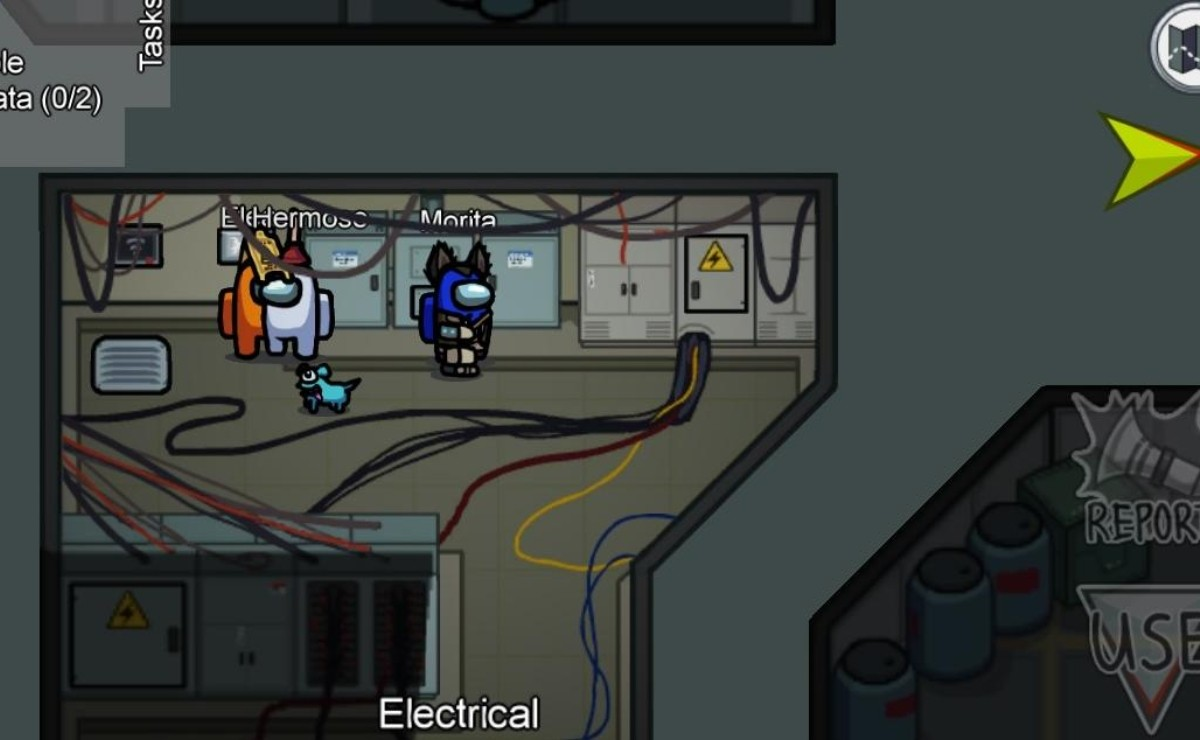
\includegraphics[width=10cm]{Among.jpg}
\centering
\caption{Referencia para la interfaz del nivel 1}
\label{fig:among}
\end{figure}

En la Figura (\ref{fig:tareas}) \cite{tareas} , se muestra una referencia de la forma como se pueden implementar las posibles tareas o minijuegos del nivel 1.

\begin{figure}[h]
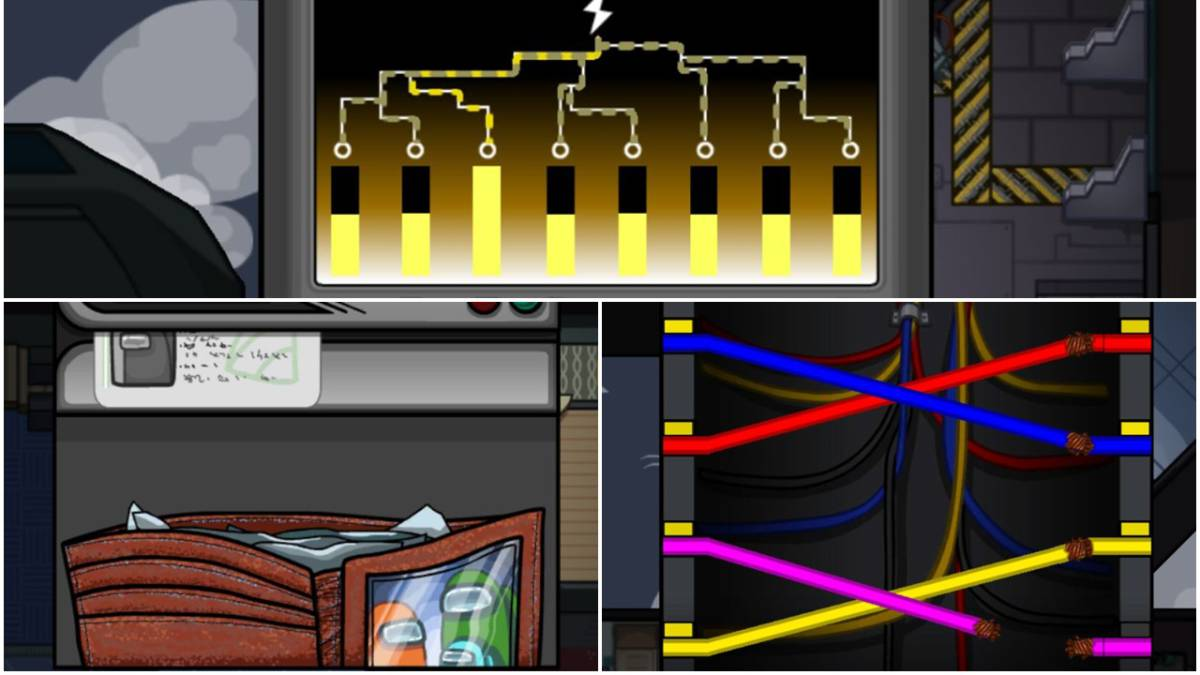
\includegraphics[width=10cm]{Tareas.jpg}
\centering
\caption{Referencia para las tareas que se desean agregar}
\label{fig:tareas}
\end{figure}

\newpage

En la Figura (\ref{fig:nivel2}) \cite{space} , se muestra una referencia de la forma como se puede implementar el nivel 2, donde se intenta llegar a salvo a la tierra.

\begin{figure}[h]
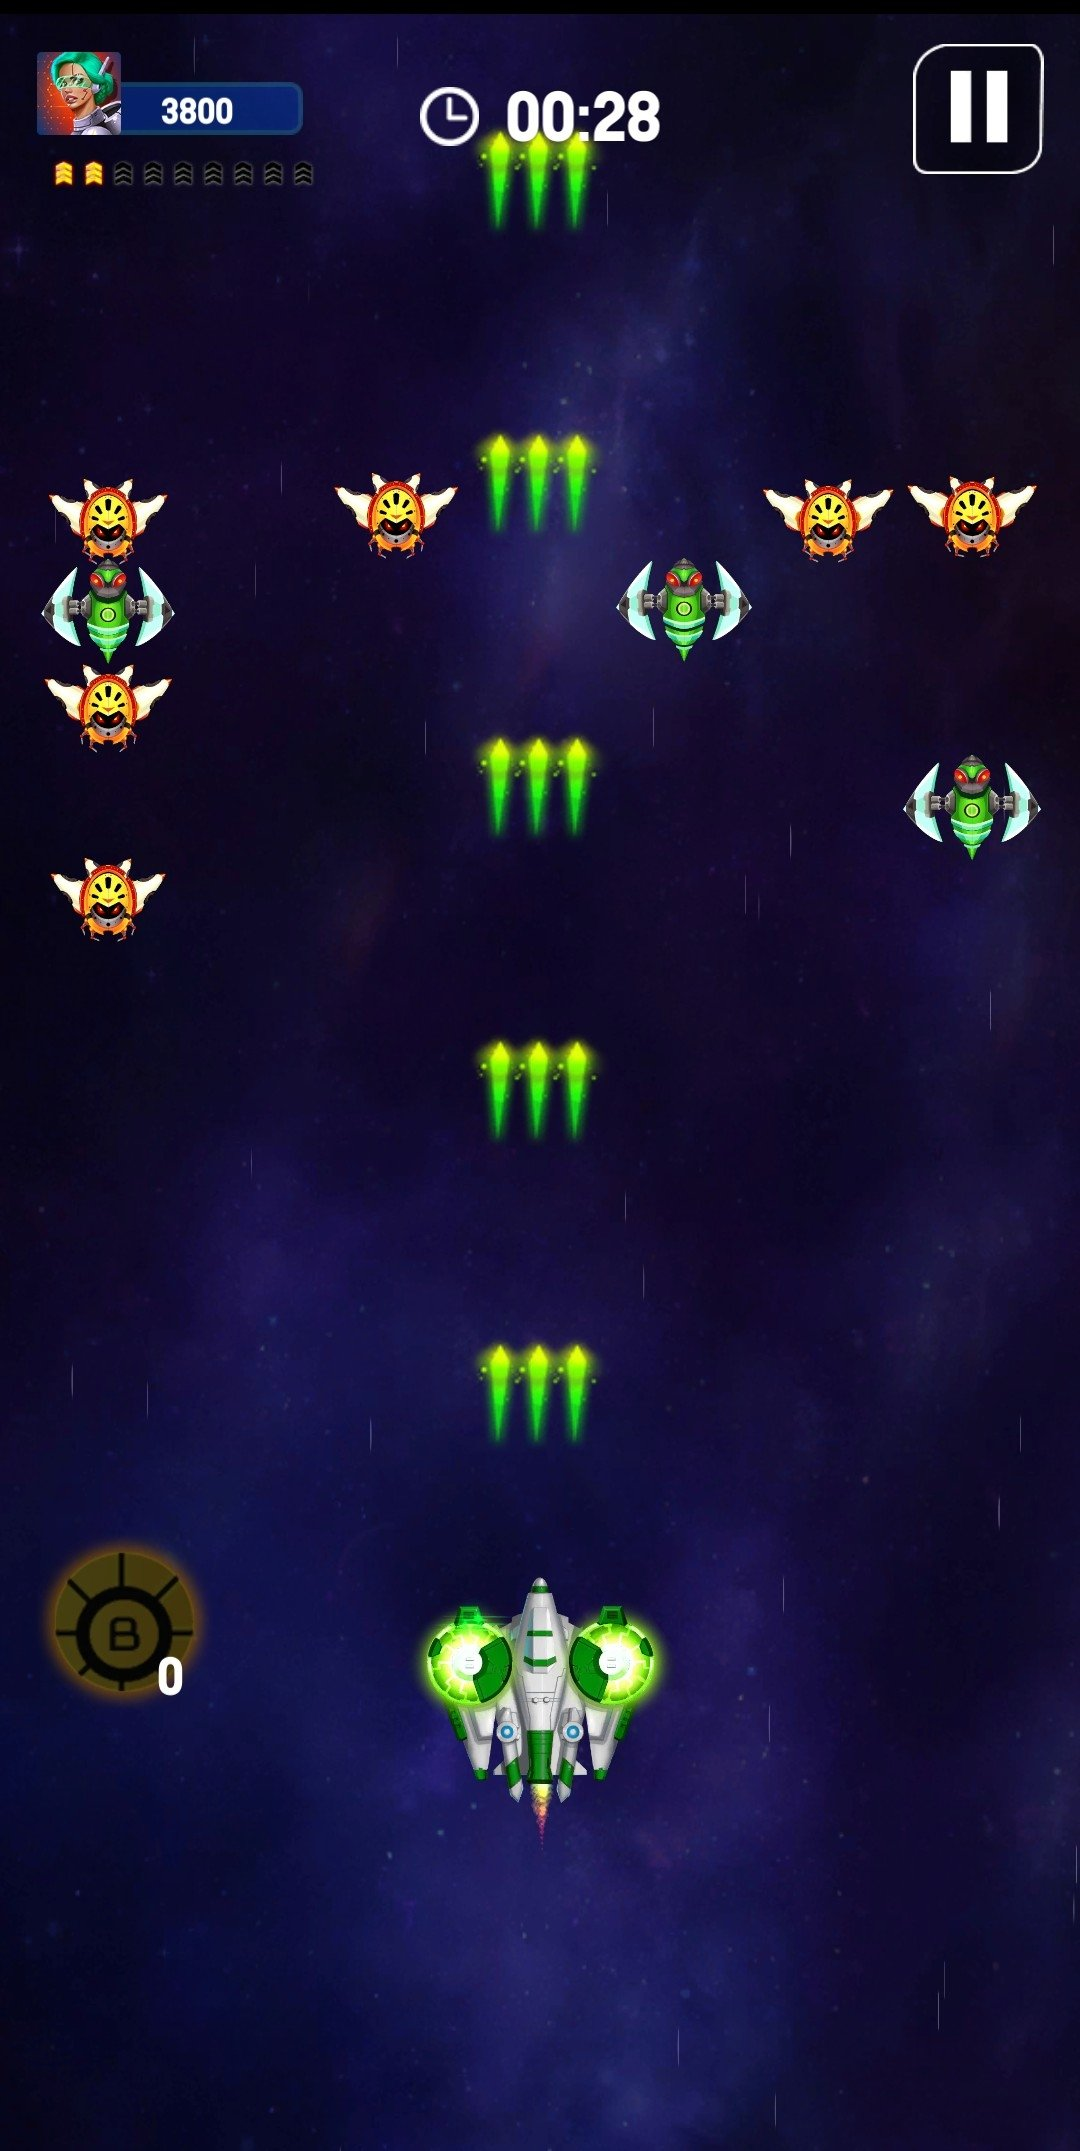
\includegraphics[width=3.3cm]{Nivel 2.jpg}
\centering
\caption{Referencia para la implementacion del nivel 2}
\label{fig:nivel2}
\end{figure}

En la Figura (\ref{fig:nivel3}) \cite{invaders} , se referencia la forma en la que se puede desarrollar el Nivel 3, donde se desembolvera una batalla en el planeta tierra.

\begin{figure}[h]
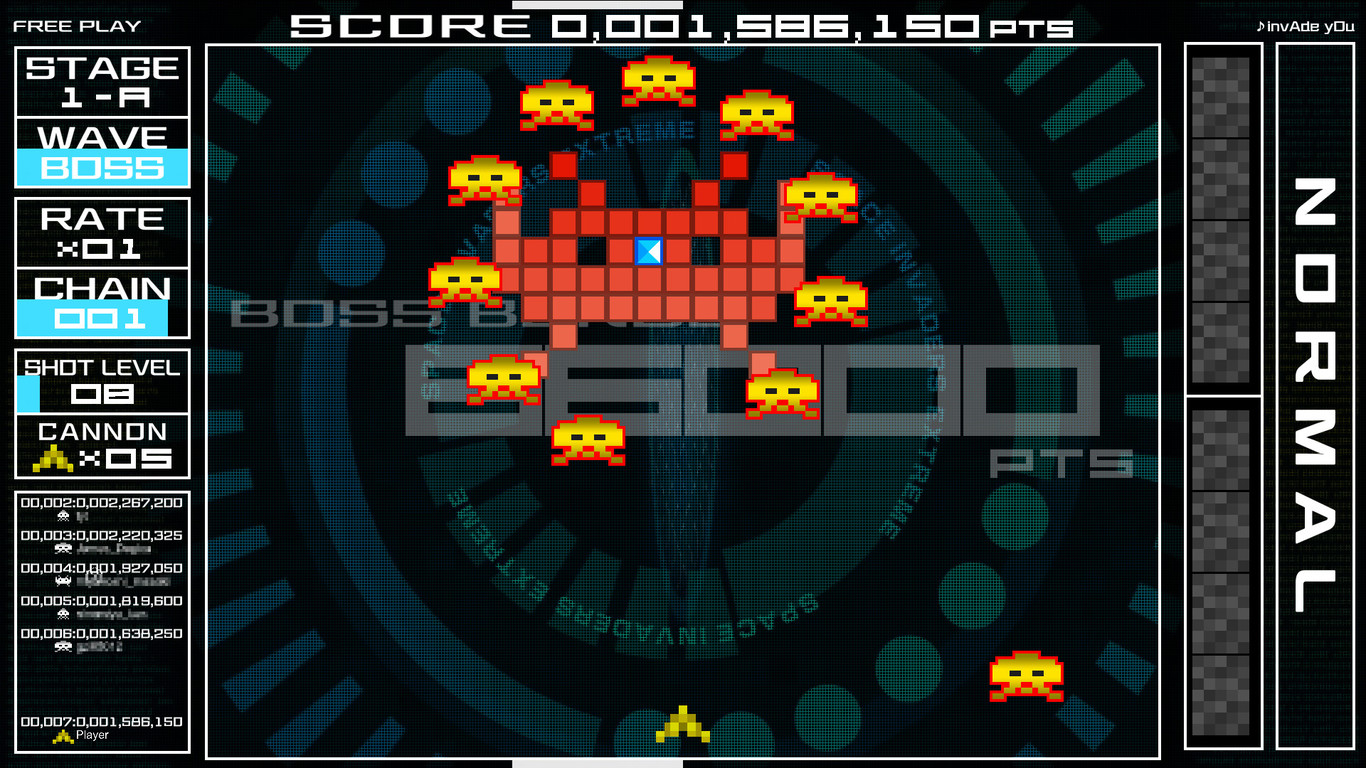
\includegraphics[width=10cm]{NIvel 3.jpg}
\centering
\caption{Referencia para desarrollar el nivel 3}
\label{fig:nivel3}
\end{figure}

\newpage

\bibliographystyle{IEEEtran}
\bibliography{references}

\end{document}
